\documentclass[tikz, border=10pt]{standalone}
\usepackage{pgfplots}
\pgfplotsset{compat=1.18}

\begin{document}
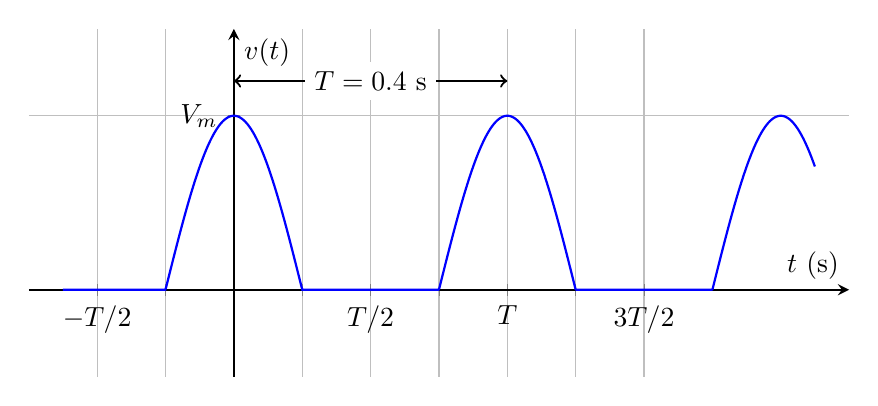
\begin{tikzpicture}
    \begin{axis}[
        width=12cm, height=6cm,
        axis lines=middle,
        xlabel={$t$ (s)}, ylabel={$v(t)$},
        ymin=-0.5, ymax=1.5,
        xmin=-0.3, xmax=0.9,
        xtick={-0.2, -0.1, 0, 0.1, 0.2, 0.3, 0.4, 0.5, 0.6},
        xticklabels={$-T/2$, , 0, , $T/2$, , $T$, , $3T/2$},
        ytick={1},
        yticklabels={$V_m$},
        grid=both,
        samples=1000,
        domain=-0.25:0.85,
        thick,
        clip=false
    ]
        % Define the function: cos(5*pi*t) if cos > 0, else 0
        % equivalent to max(cos(5*pi*deg(t)), 0)
        % For cosine, period T=0.4. omega = 2pi/0.4 = 5pi.
        \addplot[blue, thick] {max(cos(deg(5*pi*x)), 0)};
        
        % Add annotations for period T=0.4
        \draw[<->] (axis cs:0, 1.2) -- (axis cs:0.4, 1.2) node[midway, fill=white] {$T=0.4$ s};
        
        % Highlight the "rectified" nature if needed, but the plot does it.
    \end{axis}
\end{tikzpicture}
\end{document}
